\chapter{Literature Review}

\graphicspath{{./Figures/Literature Review/}}


\section{Overview of Two-Wheeled Inverted Pendulum Robots (TWIPR)}
%vertical space
\vspace{2 cm}
%figure for Ascento robot
\begin {figure}[h]
\centering
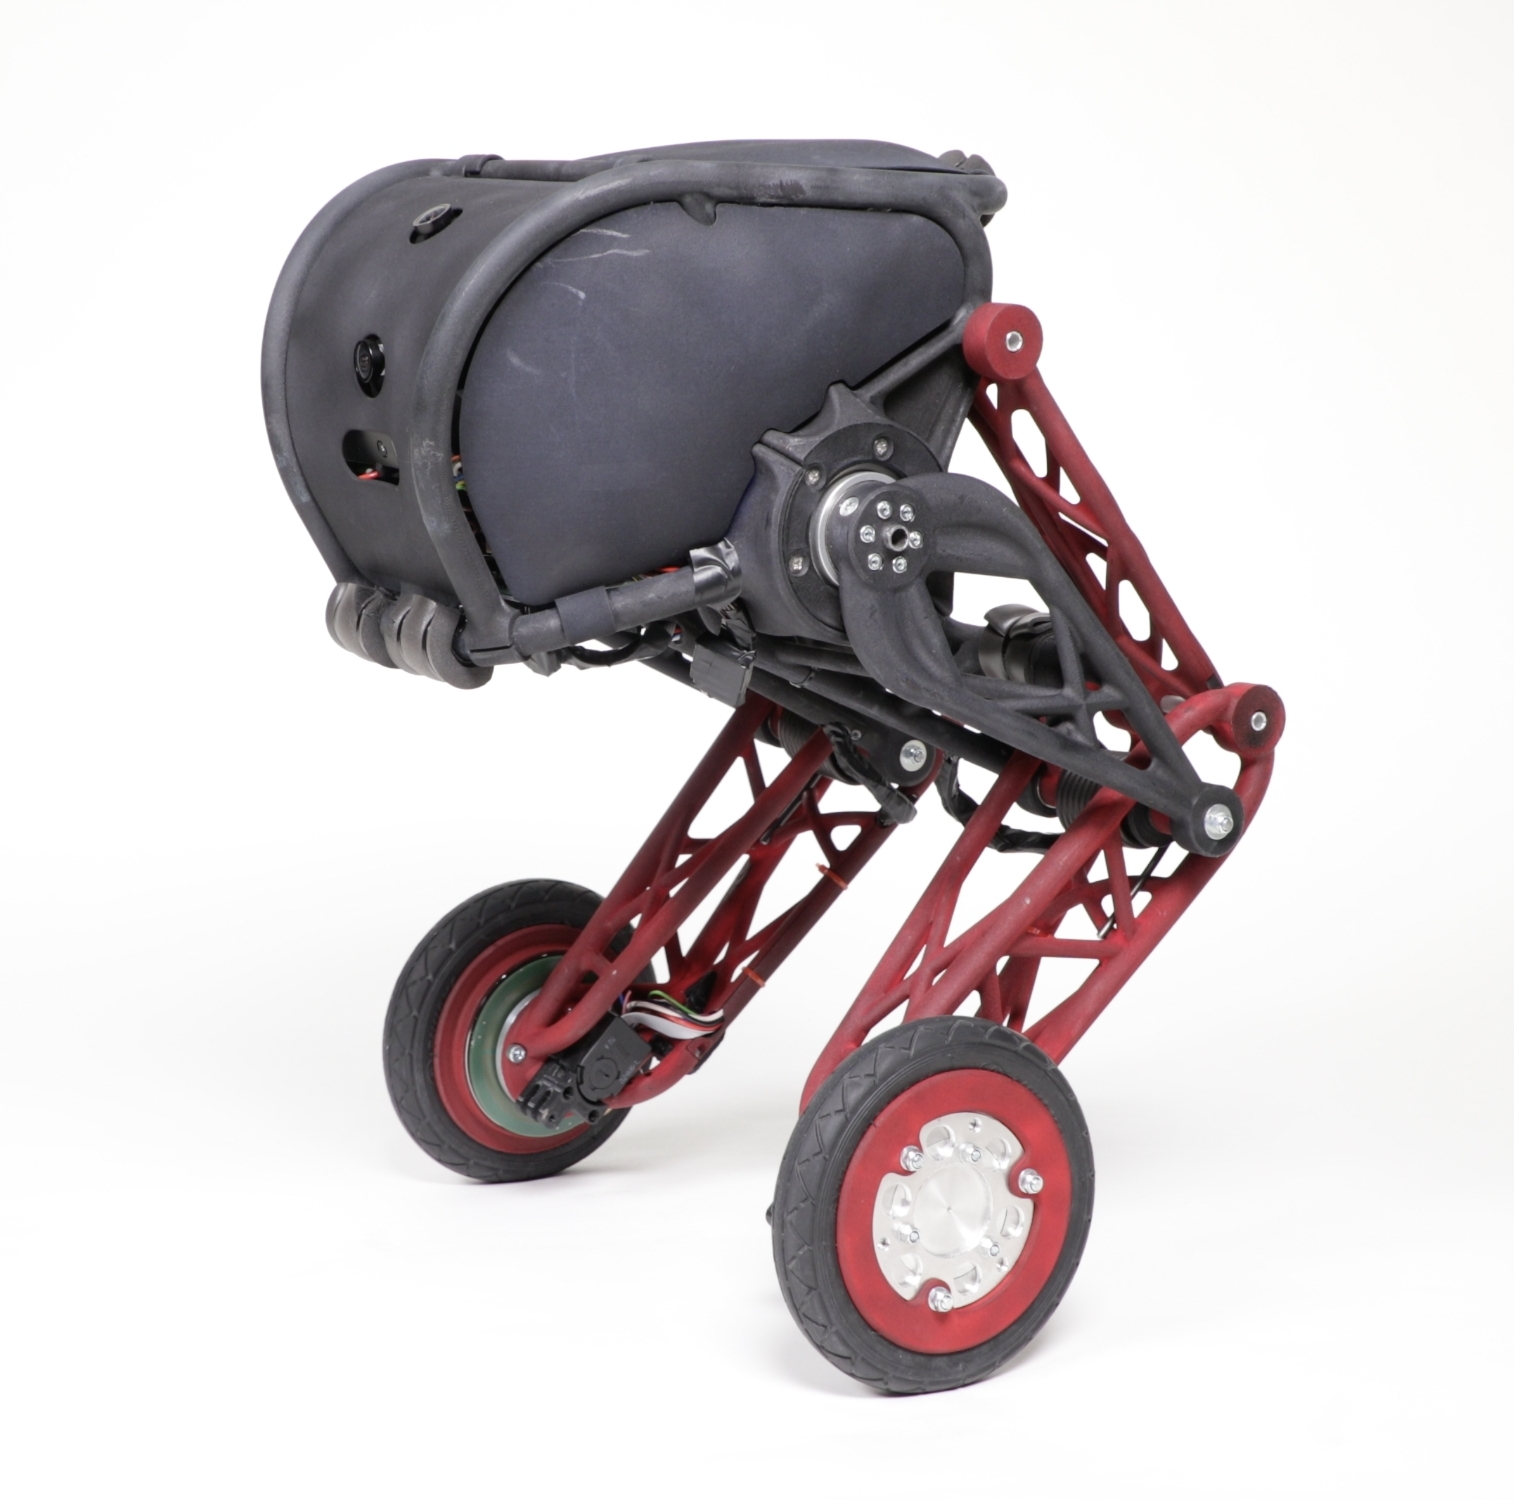
\includegraphics[width=0.5\textwidth]{Ascento robot}
\caption{Ascento Robot by ETH Zurich\cite{klemm2019ascento}}
\label{fig:Ascento robot}
\end {figure}

The Legged Two-Wheeled Inverted Pendulum Robot (LTWIPR) is a type of mobile robot that has two wheels and a body carried by two legs.
The robot acts as an inverted pendulum, with the wheels acting as the pivot point.
The robot is able to balance itself on the two wheels. The robot is able to move by tilting the body forward or backward, causing the wheels to rotate in the direction of the tilt. The robot is able to turn by moving the wheels in opposite directions. The robot is able to move in any direction by combining these movements. LTWIPRs are able to move in a variety of environments, including rough terrain and stairs. LTWIPRs are able to perform complex movements, such as jumping and climbing. LTWIPRs are able to interact with their environment, such as navigating around obstacles and diving under obstacles. LTWIPRs are able to perform tasks such as search and rescue, surveillance, and exploration.


\newpage
\section{Prior Works and Advances in Multi-Legged Robotic Systems}

%This section should provide a comprehensive review of existing literature relevant to your research topic. It should cover key theories, models, experiments, and findings in the field, particularly focusing on works that directly relate to your research question or hypothesis. This review not only shows your understanding of the field but also how your work fits into and contributes to the existing body of knowledge.
Multi-legged robots have been studied extensively in the past.
Different types of multi-legged robots have been developed such as the quadruped robots, hexapod robots, and biped robots.
\subsection{Mechanical Design and Development}
%three subfigures side by side for Honda's Asimo, Boston Dynamics' Atlas and sony QRIO
\begin {figure}[h]
\centering
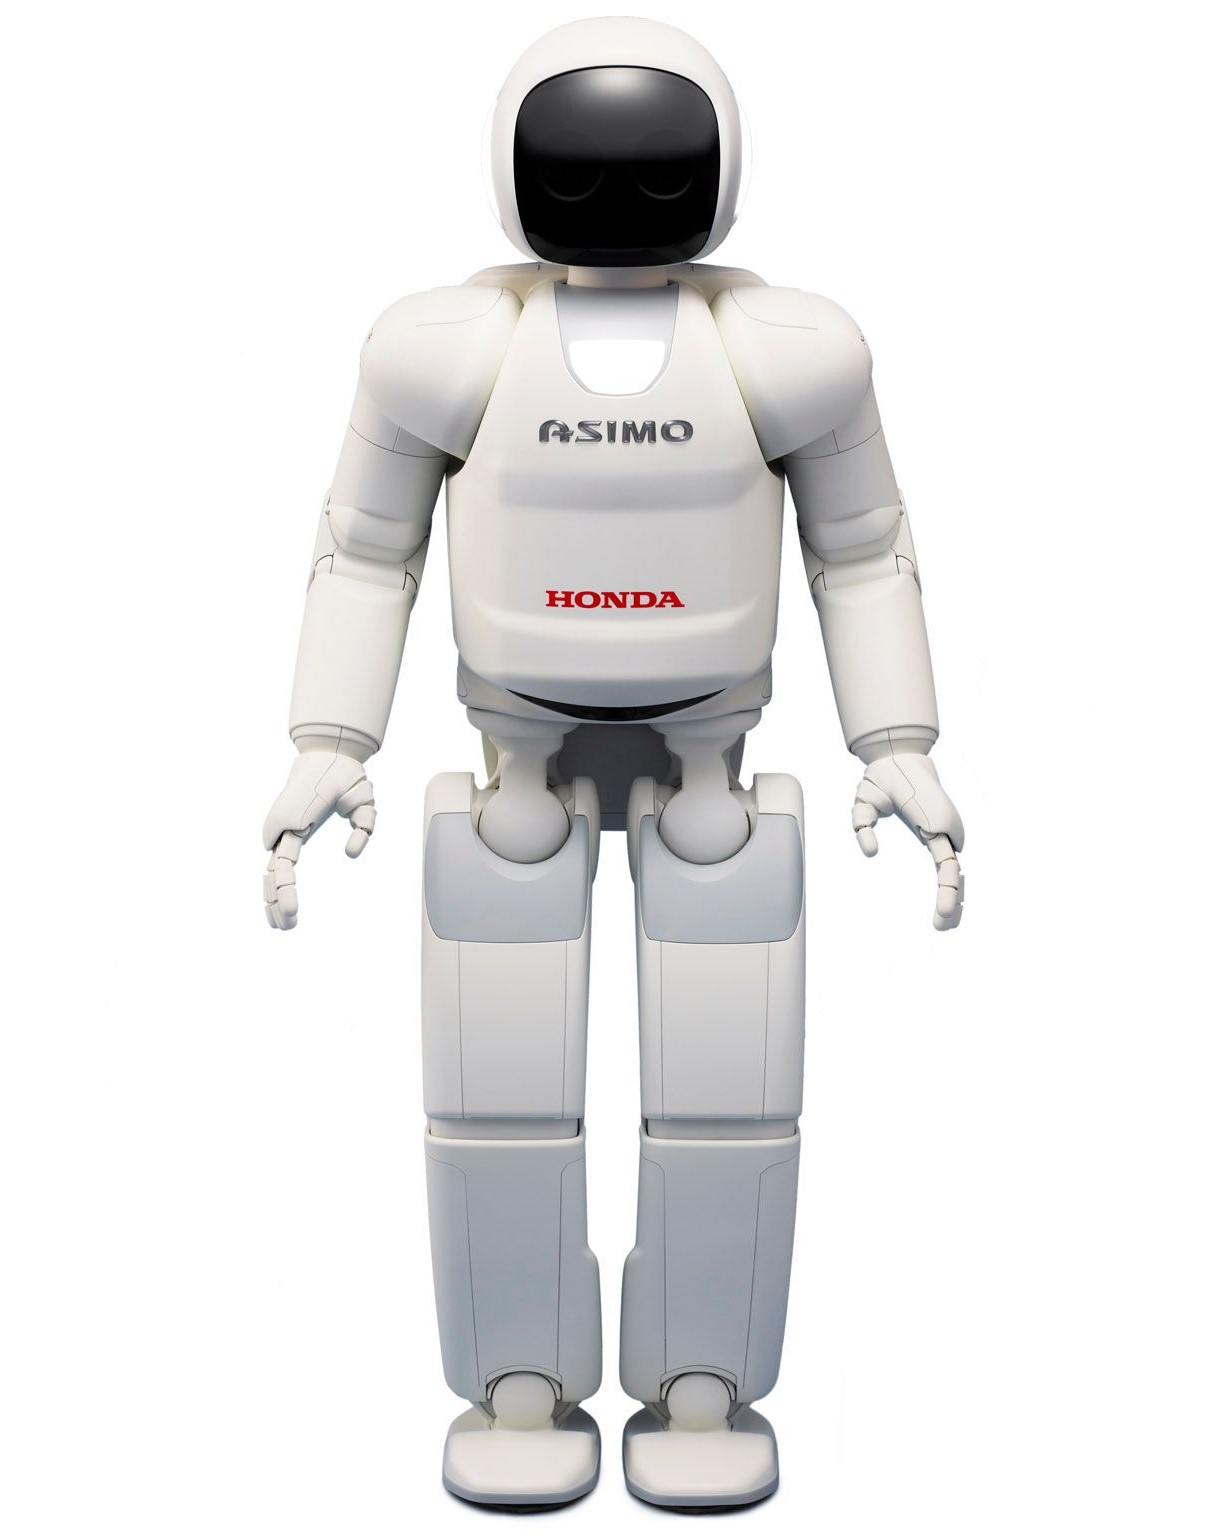
\includegraphics[width=0.3\textwidth]{Honda's Asimo}
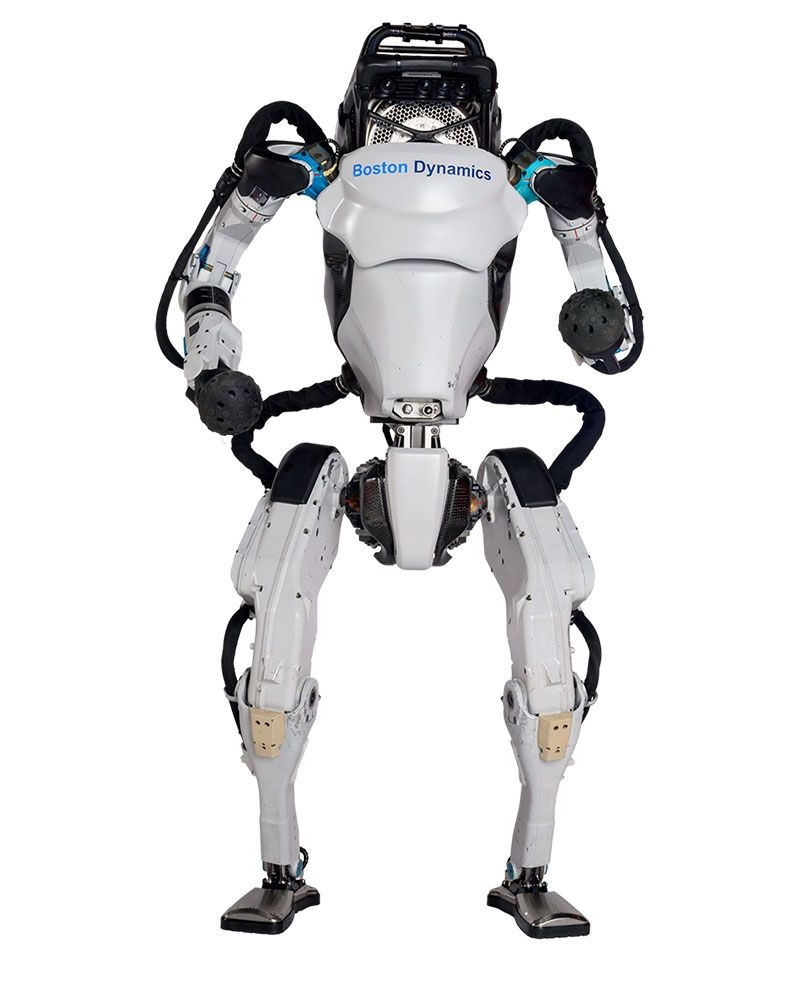
\includegraphics[width=0.3\textwidth]{Boston Dynamics' Atlas}
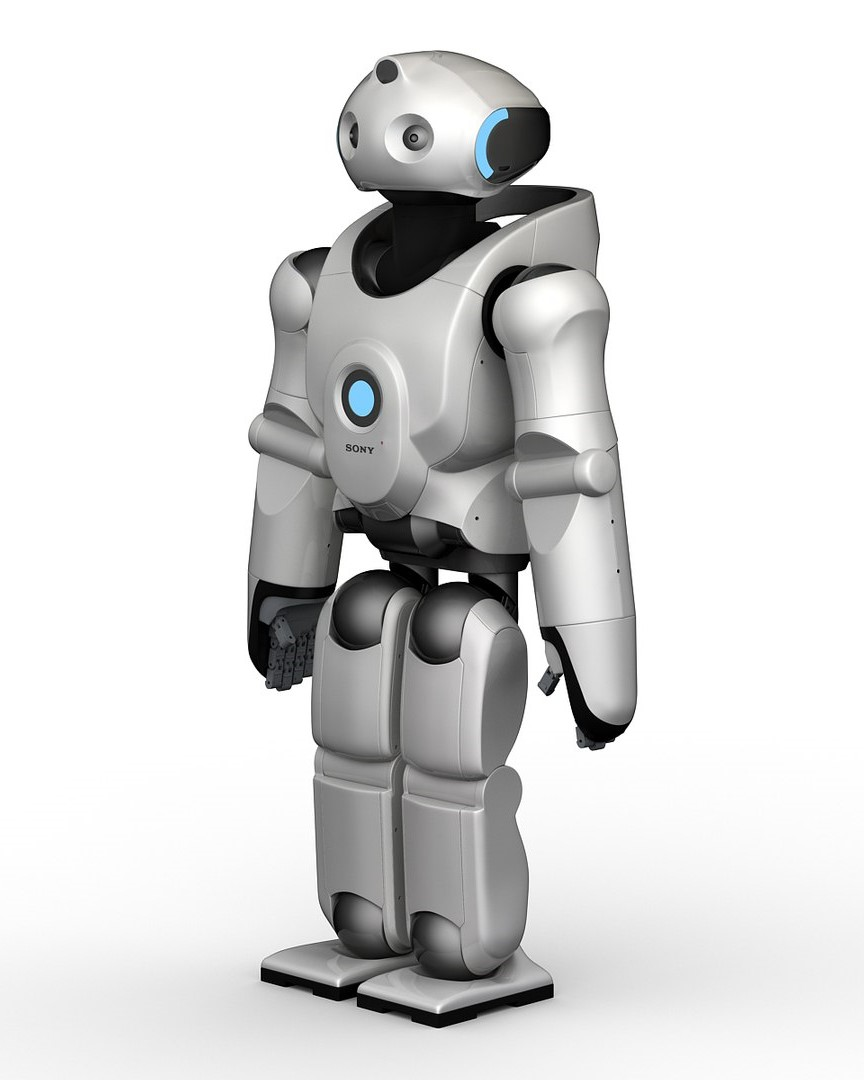
\includegraphics[width=0.3\textwidth]{sony QRIO}
\caption{Honda's Asimo, Boston Dynamics' Atlas and Sony QRIO\cite{asimo}\cite{atlas}\cite{qrio}}
\label{fig:Asimo, Atlas and QRIO}
\end {figure}


It is obvious that the mass distribution of the robot is a key factor in determining the robot's stability.
Various design considerations when designing a robot are important to consider, such as the robot's size, degree of freedom, link design, and mass distribution\cite{nath2017design}.
Biped robots have many parameters that affect their locomotion, making it difficult to determine the right design parameters to achieve stable and reliable gaits.
The purpose of designing and assembling this biped robot is to advance research on humanoid robots and to offer a platform for studies on biped locomotion.
It is simple to change the structure to suit the researcher's interests and the type of testing that must be done.
As a result, the platform requires little upkeep.
With the help of sensors, electrical actuators, and mechanical connections, biped robots with full functionality are put together to carry out a specific task.
An apparatus for processing (PU), primarily consisting of an embedded processor, which methodically regulates every part of the biped robot.
Several robots are built around these microcontrollers.
Because of the significant processing power that is contained on a single chip, programmers have a great deal of flexibility\cite{madadi2007design}.
 The design of bipedal robots is a complex task that requires a thorough understanding of mechanics, control systems, human biomechanics, and robotics software.

%figure for evoBOT-3
\begin {figure}[h]
\centering
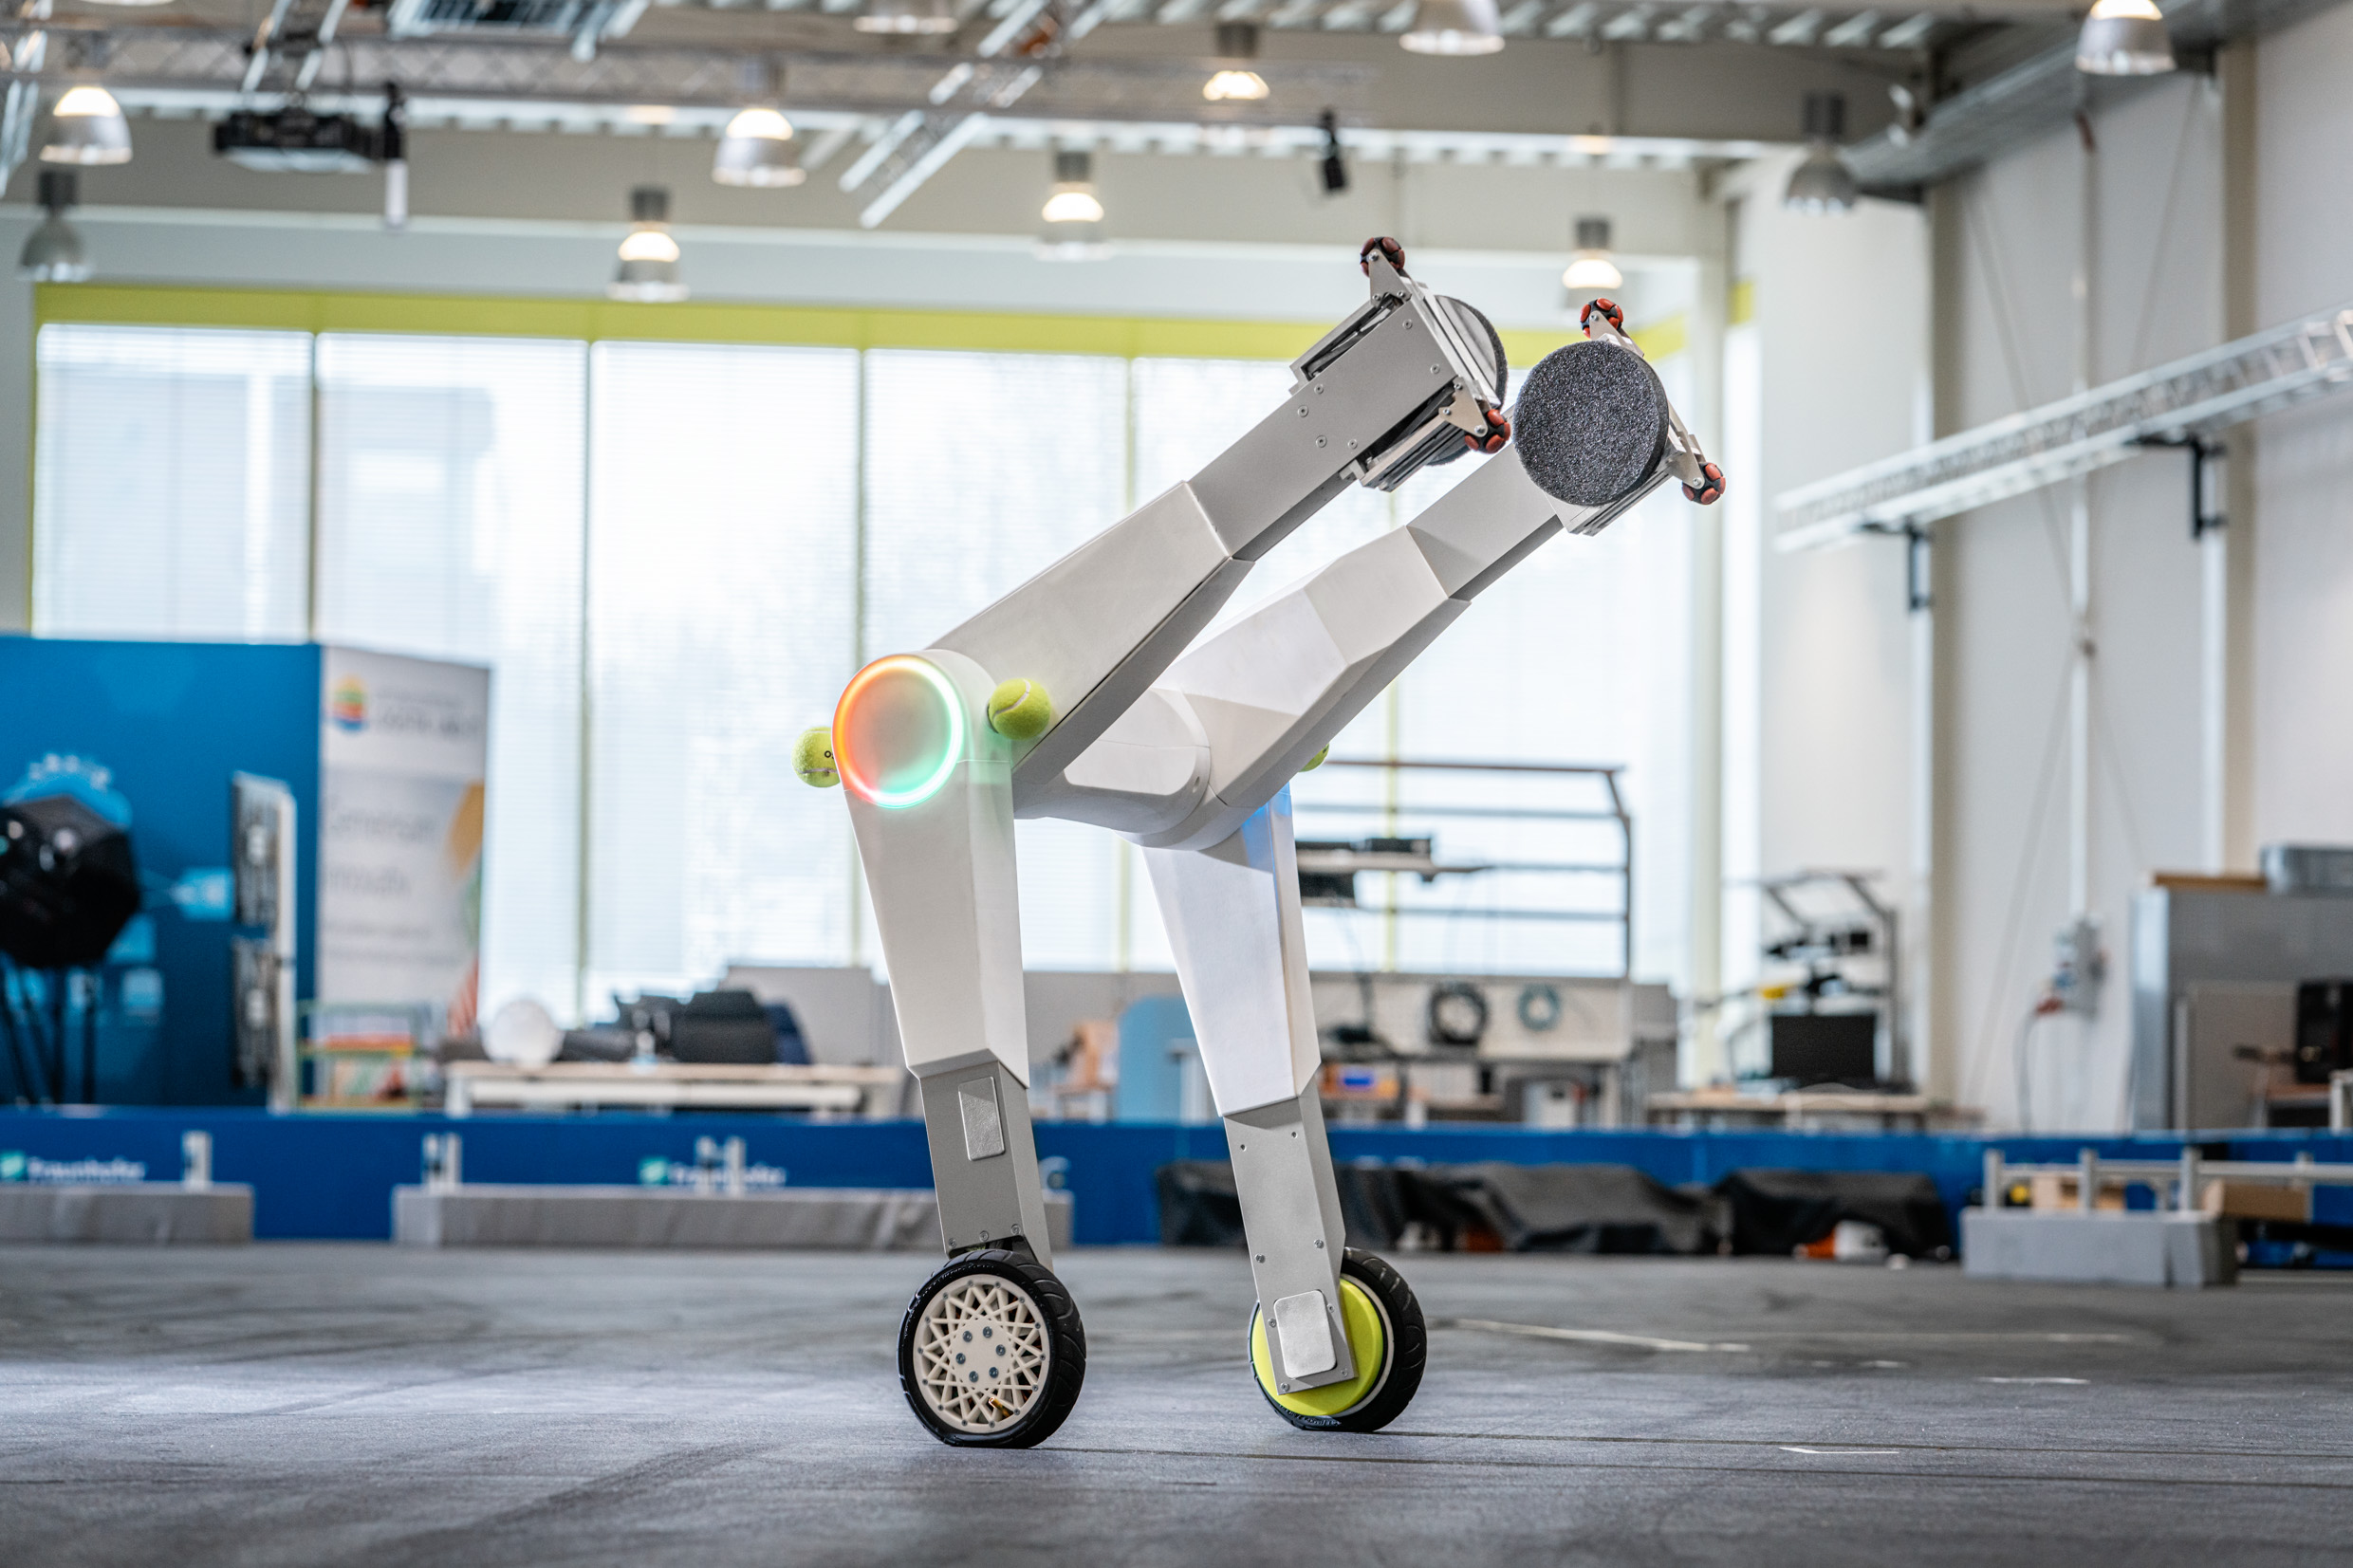
\includegraphics[width=0.5\textwidth]{evoBOT-3}
\caption{evoBOT-3\cite{klokowski2023evobot}}
\label{fig:evoBOT-3}
\end {figure}

The Legged Two-Wheeled Inverted Pendulum Robot (LTWIPR) such as the Ascento robot by ETH Zurich \cite{klemm2019ascento} and similar robots designs studied in \cite{guo2022design},\cite{zhang2022dynamic},\cite{cui2022modeling},\cite{hsu2022implementation} and \cite{xin2020online} demonstrate the different design approaches that can be used to design a LTWIPR. The wheel-leg hybrid design of the LTWIPR allows for the robot to have the advantages of both wheeled and legged robots.
another design differs, such as the evoBOT-3.
High levels of flexibility and agility define the evoBOT. This collaborative robot can be used in complex urban spaces, going beyond the traditional logistical context.
These extensions include load carriers and the passing and turning of objects.\cite{klokowski2023evobot}

\subsection{Dynamic Modeling of Wheeled Bipedal Robots}
The dynamic modeling of wheeled bipedal robots is a complex task that requires a thorough understanding of the robot's kinematics and dynamics.
 \cite{kim2015dynamic} outline the kinematics and dynamics of the Two-wheeled Inverted Pendulum Balancing
Mobile Robot where the kinematics constraints are derived and the dynamics are derived using the Lagrangian and Kane's methods.
The equations of motions derived in this work can be considered as the base for the Legged Two-Wheeled Inverted Pendulum Robot (LTWIPR) since the Two-wheeled Inverted Pendulum Balancing Mobile Robot is a generalization of the LTWIPR. Free body diagrams are also different approaches that can be used to derive the equations of motion of the LTWIPR. The study \cite{zimit2018modelling} presents the modeling for the TWSB robot using free body diagram approach.
The modeling of the robot is a critical step in the development of the robot since it is used to derive the equations of motion of the robot which are used in the control of the robot.
Good understanding of the robot's dynamics is required to develop a good control strategy for the robot.



\subsection{Control of Wheeled Bipedal Robots}
Different control strategies have been implemented on wheeled bipedal robots such as Fuzzy Logic, PID, LQR, MPC, and Reinforcement Learning.
The control strategies are chosen based on different factors such as the control objective, the complexity of the Robot's Dynamics and Requirements, The Robot's Operating Environment. In \cite{hsu2022implementation} it shows that To keep the WBR balanced while it is standing and moving on the ground, an intelligent motion and balance controller (IMBC) built on a fuzzy logic technique is suggested.
It is important to note that the suggested IMBC system does not require any prior understanding of system dynamics, and that human knowledge's qualitative components are used to adjust the controller parameters. The study \cite {cui2022modeling} shows the implementation of LQR control on a LTWIPR because it efficiently resolves the issue of striking a balance between control effort and good system response.
The wheels of the Wheel-based robot are controlled by the LQR controller because the pendulum length varies during movement.
Other studies demonstrate classical control strategies such as PID control on Two-wheeled self-balance robot.
The study \cite{zimit2018modelling}shows the implementation of PID control on a Two-wheeled self-balance robot where PID gains are tuned until ideal performance is achieved.
Some other methods such as controlled lagrangian are used to stabilize an inverted pendulum that is fastened to the end of a robotic arm that rotates\cite{bloch1999stabilization}.
Model Predictive Control (MPC) is also a powerful and versatile control strategy that has been used on wheeled self-balancing robots. \cite{azimi2013model} presents the development of model predictive control (MPC) for each subsystem of a two-wheeled self-balancing robot (TWSBR) in order to achieve a stable and robust control system. The control of the robot is an intricate process that involves advanced algorithms to achive the desired control objective.
\vspace{3 cm}
\subsection{Integration of Learning and Adaptive Control Mechanisms in Wheeled Bipedal Robots}
In the absence of an accurate dynamic model of the robot, Adaptive dynamic programming (ADP) and reinforcement learning (RL) can be used to derive an adaptive optimal control solution based on learning.
In contrast to the LQR control which requires an accurate dynamic model of the robot.
In complex mechanical structures such as the LTWIPR, the dynamics are difficult to model accurately.
Learning and adaptive control mechanisms can be used to overcome this challenge. The study \cite{cui2021learning}proposes a data-driven algorithm to generate near optimal balance control for a two-wheeled self-balancing robot.
In other research, Adaptive variable impedance control (AVIC) is used to control the robot's balance specifically in the case of interaction with complex unknown terrain\cite{xu2020adaptive}.
The AVIC controller is used to control the robot's balance by minimizing the force tracking error for each leg that is exerted on the body.
\subsection{Applications and Future Directions}
There are many applications for wheeled bipedal robots, including Agriculture, Search and Rescue, surveillance, warehouse automation, military, and others.
Further research is needed to improve the performance of wheeled bipedal robots in terms of speed, stability, and robustness.
Solutions for different problems such as the localization of the robot, the navigation of the robot, and the interaction of the robot with its environment are needed to advance the field \cite{raj2022comprehensive}.
Machine learning and artificial intelligence can be used to improve the performance of wheeled bipedal robots\cite{kuutti2020survey}.

